\documentclass[12pt]{article}

\usepackage[hyphens,spaces,obeyspaces]{url}
\usepackage{graphicx}
\graphicspath{ {./images/} }
    

\title{CMPUT 499 Literature Review}
\author{Monica Bui}

\begin{document}

\begin{titlepage}
    \centering
    \large
    \vspace{1cm}
    CMPUT 499: Mining Sofware Repositories \\
    \vspace{1cm}
    Literature Review \\
    \vspace{1cm}
    Monica Bui
\end{titlepage}

% What is the issue of paper? Main goals and questions? Methods of research? Results? Conclusion with personal opinion (good/bad/limitations).

% Literature review discusses published inforamtion in subject area
% Focus on summarizing source and introducing my own understandings of topic

\newpage
\section{Introduction}
% Give idea of the topic of the literature review, patterns + theme
% Work in Progress. This will be edited a lot.s
Third-party software libraries and Application Programming Interfaces (APIs) offer a way for developers
to use existing features and funuctionalities to build their projects without having to re-invent the wheel.
There are many libraries to use for different programming languages whether it is open source 
or hosted elsewhere. Although having this much freedom for deciding on what libraries to use is flexible,
it is also conflicting to figure out which one is best for your project. It is difficult to choose because
there are a variety of factors involved such as functionality and developer support. 
In this review, we look at several diferent articles to help analyze various properties of libraries and 
to determine a high quality method of comparison between them.

\section{Article Review}
% Not sure how to format articles. Could start with one article per paragraph.

% That would take to long. Format by theme? 
% Recommenders, Badges, API Comparisons by Metrics, Usage, etc.

\subsection{Library Recommenders}
\paragraph{}
One problem is researching new analogical libraries to use for different programming languages that has similar functionalities 
to the ones you currently know. Chen's et. al \cite{analogical} paper discusses their library recommender 
that compiles a list of libraries from community resources such as blogs and Q\&A sites like StackOverflow \cite{stackoverflow} 
and outputs a list of recommended libraries in the developer's language of choice. 

This is implemented by first mining tags on questions posted online on StackOverflow \cite{stackoverflow}.
These tags are split into two knowledge bases: relational and categorical. Respectively, relational knowledge is how pairs of
tags are correlated to each other eg. Java and JUnit while categorical knowledge consists of how tags are grouped into categories such as 
language, operating system, concept, or library with both bases being analyzed by NLP. 
The key idea here is that having different seperated tag categories and relatonships between tags often mentioned together
allowed for a simpler way to recommend a new library. With the database in place, users can then search for recomendations through the built
web application called SimilarTech \cite{similartech}.

While trying out the application myself, I found that search results would only yield for 
libraries that are mentioned in specific contexts.
Axios \cite{axios} a popular Javascript HTTP library should output expected 
recomendations like Requests \cite{requests} module for Python but the actual list printed was empty.
Axios \cite{axios} itself is mentioned around many situations like REST, APIs, and HTTP requests making it difficult to figure out in what context it should be recommended.

While the number of languages it can suggest libraries for is limited to 5, the precision metric is impressive
with 1 language at 81\% and with 5 being at 67\% showing its potential to grow in the future.

\paragraph{}
Going back to the key problem of deciding on the right library to use, Uddin's et. al \cite{opinerarticle} article
highlights their approach to this by looking at personal developer opinions's on different resources
and how it affects the reader's decision. Furthermore, the sentiment behind this can be used to indicate if its 
a positive, questionable, or a negative API to use. The tool created, Opiner \cite{opiner} is a summarization engine
that examines these opinions and evaluates its sentiment to see if the API should be recommended also displaying ratings on API traits
and organizing top opinions on both positive and negative sides. 

The backend of the application web crawls through a Q\&A site, StackOverflow \cite{stackoverflow} to extract answer
information surrounding an API topic. This data is used to help discover when an API in mentioned, what kinds of opinion
are associated with an API, and combining these opinions under common aspects developers care about such as usability and performance.

Using Opiner \cite{opiner} through a small research study evaluated on 2 seperate groups of particpant's choices to see if 
just StackOverflow \cite{stackoverflow} alone would work for decision making on selecting an API or both StackOverflow and Opiner would be better.
We view that devlopers are more confident in their selection with both tools vs just StackOverflow alone. 

A weakness is that although the evaluation of the study proves useful, having 100\% as a percentage for using both StackOverflow and Opiner
would be hard to generalize for a larger population. 

\subsection{Github Badges}
\paragraph{}
Many developers like to both use and contribute to open-source software projects on GitHub \cite{github}. 
With many online software to use, it's difficult to pin point which is worth your time to contribute to and integrate with your project.
Trockman et. al \cite{githubbadges} looks at the in depth quality of a package by analyzing repository badges eg. Figure \ref{phpbadge} that maintainers display on their README.

\begin{figure}
    \centering
    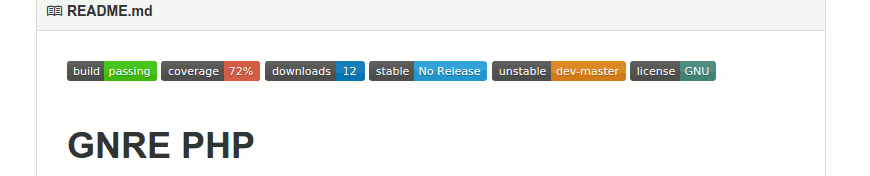
\includegraphics[width=\textwidth,height=6cm,keepaspectratio=true]{gnrephpbadges}
    \caption{
        Example badges in a open source PHP repository \protect\cite{badgeimage}
    }
    \label{phpbadge}
\end{figure}

Trockman not only mentions that badges are signals to make qualities of a project more transparent but also "may impact users' and contributers' decision making" \cite{githubbadges}.
Game like elements known as \textit{Gamification} are not explicitly embedded into these badges but in reality motivate users to contribute higher quality code to increase the signal quality
displayed by these visuals. 
The key questions to ask are, \textit{What are the most common badges and what does displayong them intend to signal?} and \textit{To what degree do badges correlate with qualities that developers expect?} \cite{githubbadges}.
To examine the impact of badges, Node Package Modules (npm) \cite{npm} is used as the research repository as it's the largest online collection of Javascript packages. 

% Research method analysis
Data is collected by mining all npm \cite{npm} packages and keeping those with metadata that included 
important metrics and a public Github \cite{github} repository. They extract the badges through the git history associated with 
the README file by matching the regular expression for a badge insertion then further categorizing them into specific categories
such as quality assuracne, popularity, dependencies etc. which each have different signaling intentions.
With their survey insights, they develop sub questions to validate the qualities the badges are supposed to show. 
For each type of signal (dependencies, popularity, test suite, and quality pull requests), they look at 
impact before and after badge adoption through longitudinal analysis, statistical regressions
to see how it is correlated with their arguments, and any underlying indicators that the badge may not overly express at first glance.

% Results and conclusion
The results suggest that displaying badges highly correlate with better code practices specifically higher test coverage, updated dependencies, and higher quality code.
However, overwhelming your repository with badges loses its intended signaling effect thus turns away users leading to decrease in downloads.
Assessment signals that are more costly to produce are more reliable than static conventional badges that display trivial information already readily found on the page.

% My opinions
With their survey design research method that collected important libraries metrics from contributers and maintainers however, having such a low response rate of 15.3\% 
is difficult to generalize that these results will stay reliable for future studies.

% look for main motivation behind project, goals, why they looked only at these prospects.
% evidence for why this method is better


\subsection{Metrics}
\paragraph{}
% API popularity and migration
With software libaries and APIs evolving at a rapid speed, upgrading to the latest software can be cumbersome for developers
as challenges of backwards incompatability and deciding on new APIs for your project prove to be a problem.
Hora et. al \cite{apiwave} dicusses these 2 obstacles and implements a web application \textit{apiwave} \cite{apiwavewebsite} to mitigate these problems and
highlight API popularity and migration in depth with the former measured by the number of users using the service.

The research method takes the Git history code of a repository and outputs information about the API's popularity metric, method of migration with code snippets as examples.
This code is further extracted by its Git diff. Based on the insertions and deletions, we can detect which lines have been modified for migration 
and update the popularity statistic by 1 suggesting that the old library lost a follower and the new library gained one with further 
assistance of mining import statements to see which APIs have changed.
The client side of \textit{apiwave} \cite{apiwavewebsite} can present a library at many levels including specific interface lookup eg. java.util vs java.util.Map.
\textit{Apiwave} also displays addition and deletions statistics, overall popularity graph, 
and code snippets that highlights recommended libraries to transfer over to based on diffs.

These results indicate different popularity trends and has been able to answer real life StackOverflow \cite{stackoverflow} 
questions regarding API migration. This helps to recommend the best software to use for developers based on ease of use through migration
and the number of others who support this -- popularity.

Even though there are a high number of vistors on the page, it is only limited to Java at the moment even though there are many lanugages out there
such as Javascript and Python that host many open source libaries. 


\paragraph{}
Selecting the best suited library for your work is often difficult as you need to make sure that they are not only reliable but also contain your desired features.
Mora et al. \cite{metrics} creates a method of comparison between libraries on a set criteria of metrics to help developers
compare and contrast between different software. Mentioned in the article, Uddin et al. \cite{analogical} proves that aspects
such as performance, documentation, and usability also highlighted in Trockman's et al. \cite{githubbadges} argument are
popular points to look for in an API.
Providing a quantative measure that looks at library qualities could lead to the best decision on library selection.
Key questions to look at are how to compile this dataset, and finding metrics that express the underlying quality of the library that developers care about.

Data is collected from Stack Overflow \cite{stackoverflow}, a Q\&A resource, with source code and issues found on GitHub \cite{github} all to provide
diversified content to see the perspective of API qualities at all angles. Many metrics eg. Release frequency, Performance presented by Mora et. al \cite{metrics} are also
dicussed previously by other authors \cite{apiwave,analogical,githubbadges,opinerarticle}.
For each metric a detailed description is given on what the metric portrays, how this metric is calculated by git commit extraction or previous related research by other authors,
and how it supports the method of comparison.

The web application displays detailed information all at one place to showcase the different metrics for each API. 
Although there is no audience feedback within the article, Mora et al. \cite{metrics} gives specific future prospects on how
to improve the application looking into survey feedback and dynamic updates to the information displayed. 

The study is limited to further generalization to show that quanitative measures work without specifying tests in the article. 
It also wasn't clear at first how the data is extracted at first but later found that the methodology itself has been borrowed by another author to apply to more metrics.
A detailed technical summary on data extraction could also be given to help connect the dots in the research method.


\newpage 
\section{Conclusion}
% Summarize key points
% Decide based on results from article, the method of reseach to dive into with my project
\paragraph{}
Deciding between different APIs in various libraries and frameworks proves to be challenging. 
Chen et al. \cite{analogical} and Udin et al. \cite{opinerarticle} look at explicitly recommending libraries through their web application with the latter 
focusing on opinion sentiment. Trockman et al. \cite{githubbadges} examines the impact of GitHub \cite{github} badges and whether they affect developer choices.
Finally, Hora et. al \cite{apiwave} and Mora et. al \cite{metrics} analyze quantitative statistics on API metrics with the former focusing on popularity and migration.

\paragraph{}
For future software metric research based on popular metrics found by Mora et. al \cite{metrics}
and Trockman et al. \cite{githubbadges}, we hope to create high quality, assessment Github \cite{github} badges
based on the most popular metrics to help recommend the best libraries for users through first
glance at the README file. Spending more effort on these assessment badges in addition to taking the most popular metrics 
will ensure that the impact on code quality increases
but does not overload the user with too much information on the page. 

\newpage
\bibliographystyle{IEEEtran}
\bibliography{literature_review}
\end{document}